\documentclass[mathserif]{beamer}

\usepackage{beamerthemesplit} % TODO: use different beamer theme
\usepackage{framed}

\title{SIAM: Getting Started with \LaTeX}
\author{Matthew Michelotti}
\date{\today}

\renewcommand{\arraystretch}{1.1}

\begin{document}

\frame{\titlepage}

\begin{frame}[fragile]
  \frametitle{What is \LaTeX{}?}

  \begin{itemize}
  \item \LaTeX{} is a high-quality typesetting system
  \item \LaTeX{} markup is converted into nice looking pdf files
  \end{itemize}

  \begin{minipage}{.38\textwidth}
  \begin{framed}
    \tiny
    \begin{verbatim}\documentclass[12pt]{article}
\usepackage{amsmath}
\title{\LaTeX}
\date{}
\begin{document}
  \maketitle
  \LaTeX{} is a document
  preparation system for the
  \TeX{} typesetting program.
  It offers programmable desktop
  publishing features and
  ...
  \begin{align}
    E &= mc^2 \\
    m &= \frac{m_0}
      {\sqrt{1-\frac{v^2}{c^2}}}
  \end{align}
\end{document}\end{verbatim}
  \end{framed}
  \end{minipage}
  $\rightarrow$
  \begin{minipage}{.55\textwidth} 
  \begin{framed}
    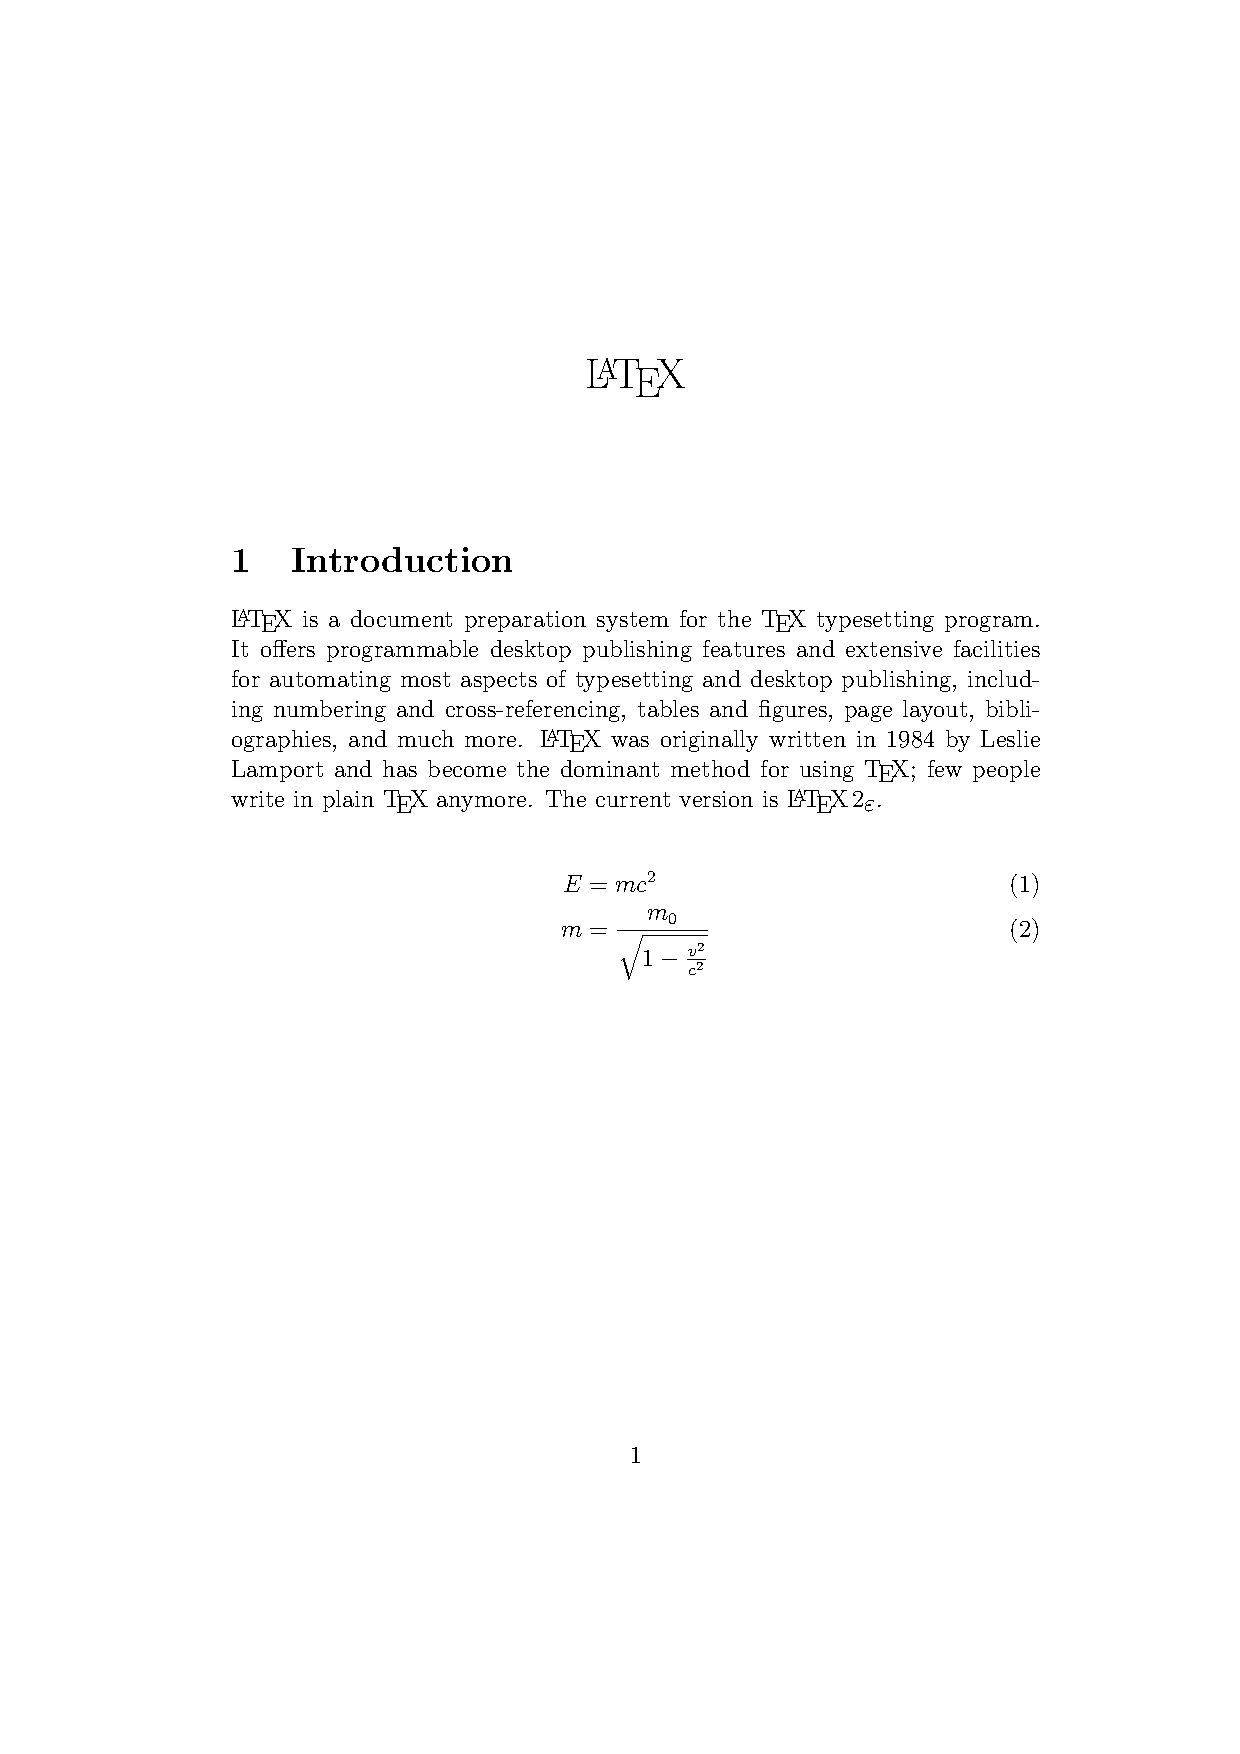
\includegraphics[trim = 33mm 127mm 33mm 59mm, clip, width=\textwidth]{figures/example_article.pdf}
  \end{framed}
  \end{minipage}
\end{frame}

\begin{frame}[fragile]
  \frametitle{Why Use \LaTeX{}?}
  \begin{itemize}
    \item Produces high-quality documents
    \item You have precise control over how document looks
    \item Excellent for typesetting mathematics
    \item Automated page numbers, section numbers, references, citations, etc.
    \item Widely used for academic journals
    \item Free
    \item Multi-platform
  \end{itemize}
\end{frame}

\frame{
  \frametitle{Exercise 1: Compiling}
  \begin{itemize}
    \item Go to website www.compileonline.com/try\_latex\_online.php
    \item Compile the example \LaTeX{} file on this website
    \begin{itemize} \item The result should look as follows: \end{itemize}
  \end{itemize}

  \centerline{
  \begin{minipage}{.6\textwidth} 
  \begin{framed}
    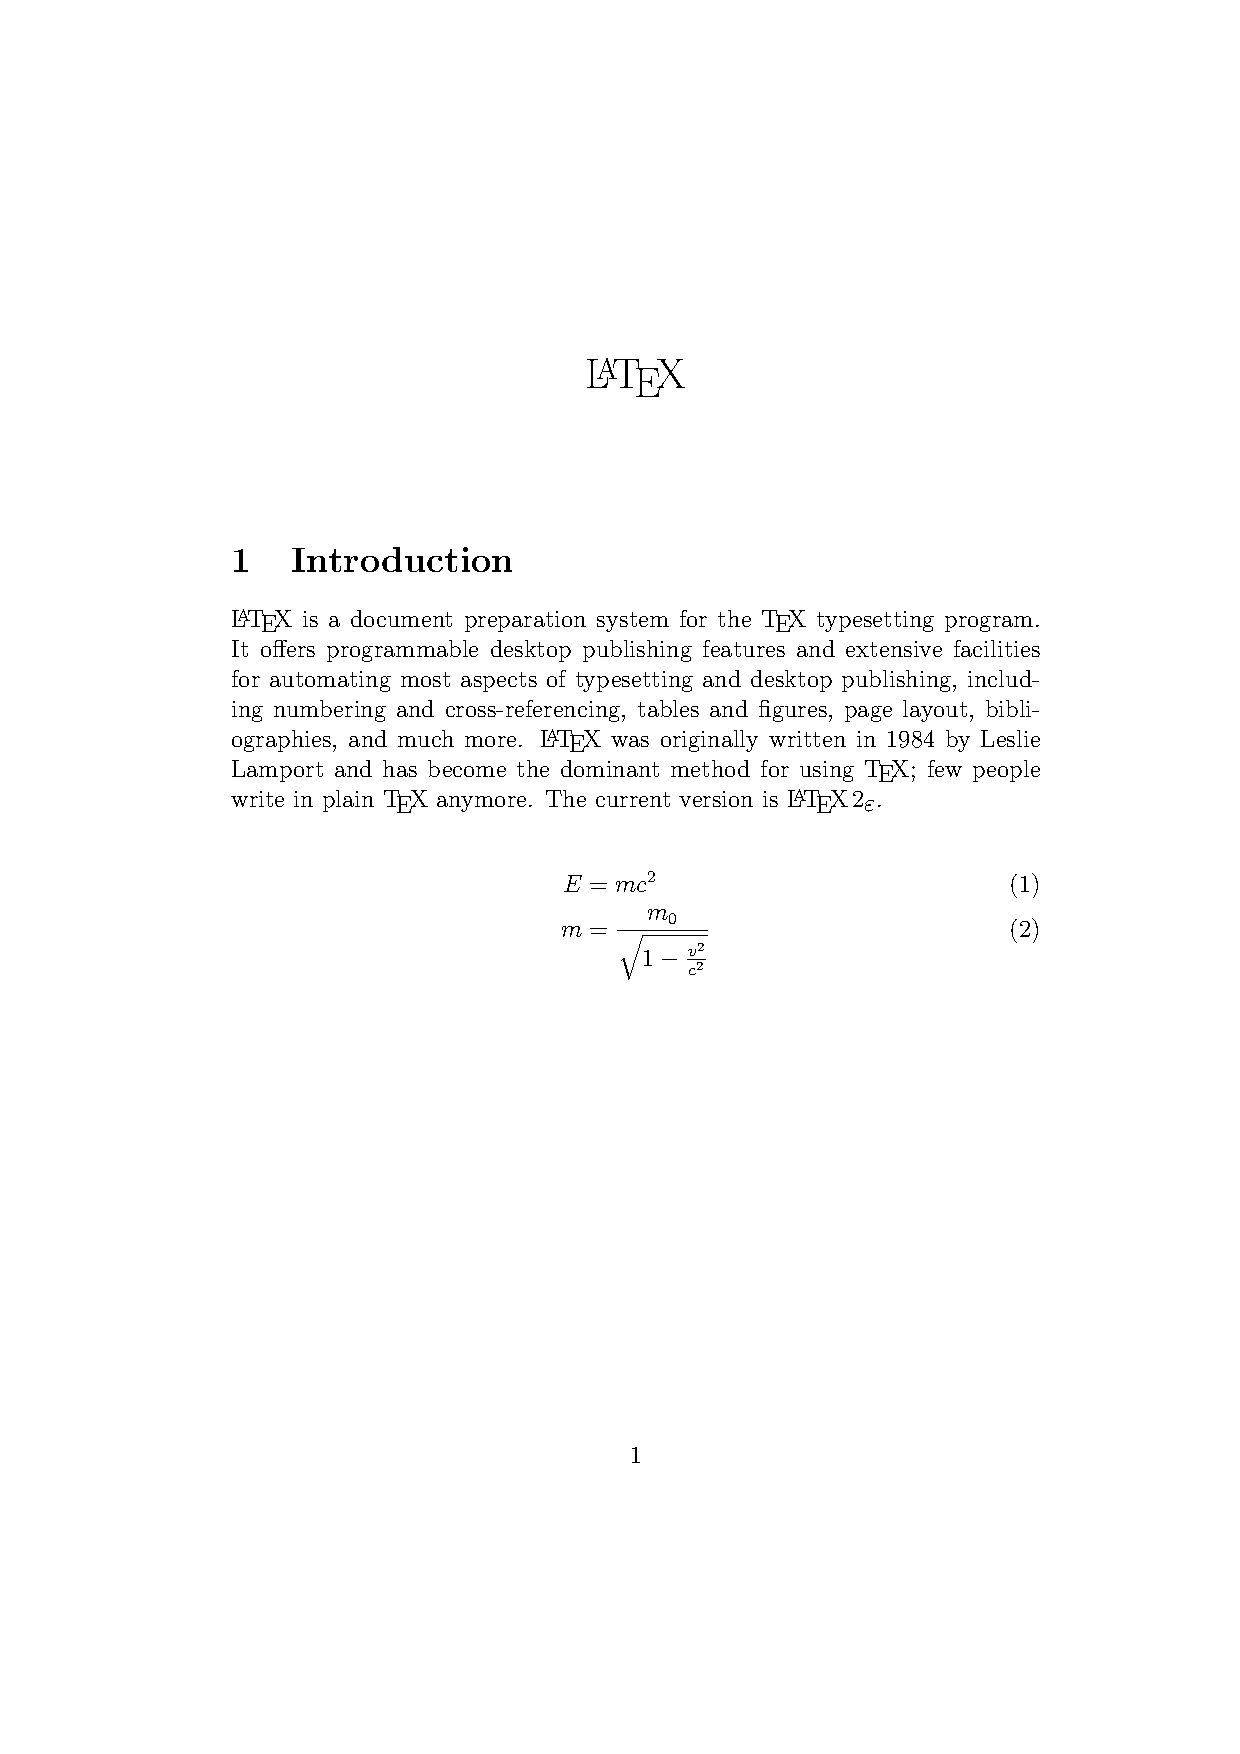
\includegraphics[trim = 33mm 127mm 33mm 59mm, clip, width=\textwidth]{figures/example_article.pdf}
  \end{framed}
  \end{minipage}
  }
}

\begin{frame}[fragile]
  \frametitle{Spaces}
{\small
\begin{verbatim}You can use LaTeX to typeset regular text.     In LaTeX,
using extra spaces       or      a newline   doesn't matter.

However,
using         two newlines in       a row
results in a new paragraph.\end{verbatim}
}
  \begin{minipage}{\textwidth} 
  %\begin{framed}
    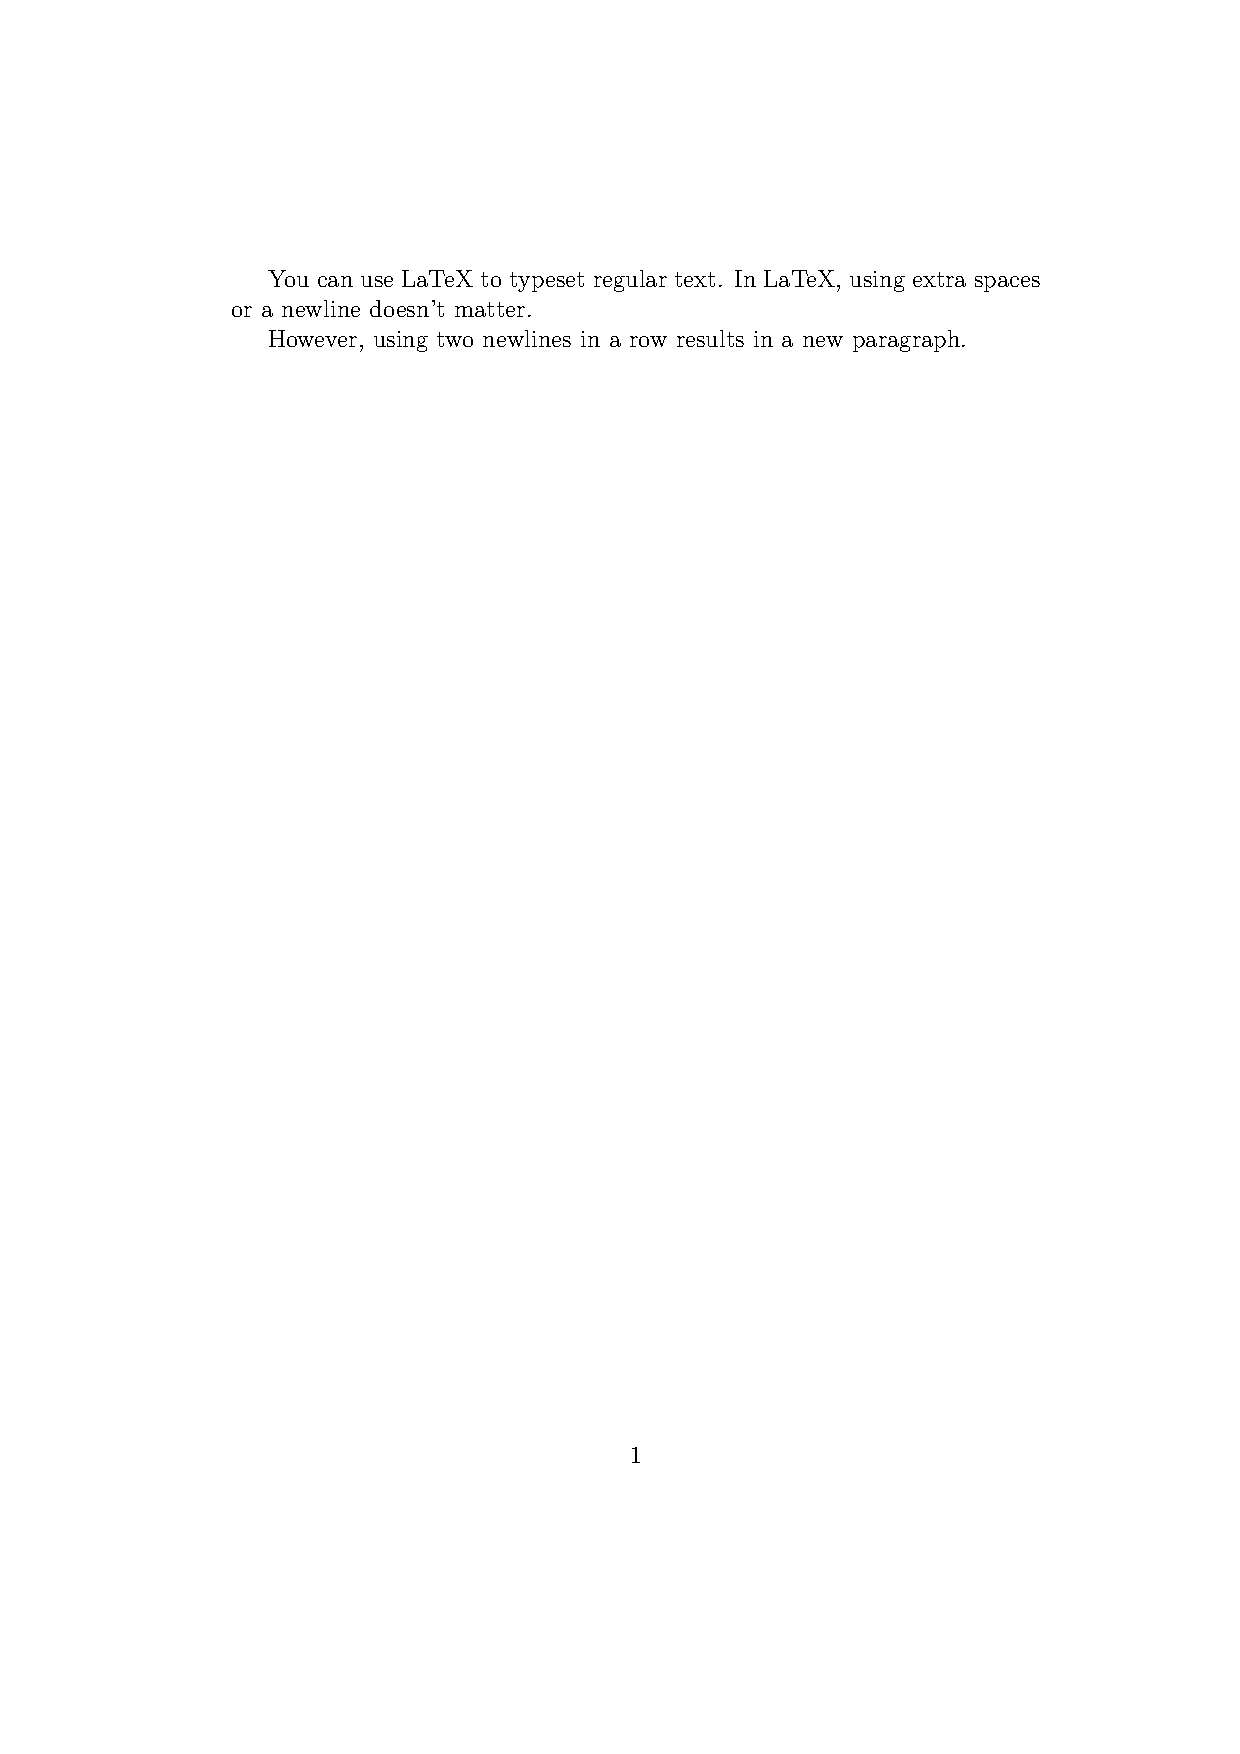
\includegraphics[trim = 33mm 230mm 33mm 40mm, clip, width=\textwidth]{figures/example_spacing.pdf}
  %\end{framed}
  \end{minipage}
\end{frame}

\begin{frame}[fragile]
  \frametitle{Control Sequences}
  \begin{itemize}
    \item \LaTeX{} uses control sequences to achieve special functionality
    \item Control sequences start with a backslash \verb|\|
  \end{itemize}
  \small
  \begin{tabular}{l l}
    \verb|\documentclass[12pt]{article}| & describes appearance of document \\
     & (similar to CSS) \\
    \verb|\begin{document}| & begins document environment \\
    \verb|\section{Section Title}| & starts a new section \\
    \verb|\subsection{Subsection Title}| & starts a new subsection \\
    \verb|\LaTeX{}| & displays \LaTeX{} \\
    \verb|\end{document}| & ends document environment
  \end{tabular}
\end{frame}

\begin{frame}[fragile]
  \frametitle{Math Mode}
  \begin{itemize}
    \item Text between dollar signs \verb|$...$| will use math mode
    \item Many control sequences only work in math mode
    \item Can use \verb|^| for superscripts and \verb|_| for subscripts
  \end{itemize}
  \begin{tabular}{l l}
    \verb|$y = 3x - 4$| & $\rightarrow \quad y = 3x - 4$ \\
    \verb|$\theta \Theta \omega \Omega$| & $\rightarrow \quad \theta \Theta \omega \Omega$\\
    \verb|$\sqrt{x} = x^{1/2}$| & $\rightarrow \quad \sqrt{x} = x^{1/2}$\\
    \verb|$\min \{ x_1, x_2, x_3 \}$| & $\rightarrow \quad \min \{ x_1, x_2, x_3 \}$
  \end{tabular}
\end{frame}

\begin{frame}[fragile]
  \frametitle{Displayed Math}
  \begin{itemize}
    \item Example: {\small \verb|f(x) = \sum_{i=1}^{\infty} \frac{1}{g_i(x)}|}
    \item Use dollar signs \verb|$...$| for inline math
      \begin{itemize} \item The equation $f(x) = \sum_{i=1}^{\infty} \frac{1}{g_i(x)}$ is displayed inline \end{itemize}
    \item Use escaped brackets \verb|\[...\]| to display math on its own line
      \[ f(x) = \sum_{i=1}^{\infty} \frac{1}{g_i(x)} \]
    \item Use \verb|\begin{equation}...\end{equation}| for automatically numbered equations
      \begin{equation} f(x) = \sum_{i=1}^{\infty} \frac{1}{g_i(x)} \end{equation}
  \end{itemize}
\end{frame}

\begin{frame}
  \frametitle{Exercise 2: Definition of Derivative}
  \begin{itemize}
    \item Produce the following equation in \LaTeX{}:
    \[ \frac{\mathrm{d}f(x)}{\mathrm{d}x} = \lim_{\delta \to 0} \frac{f(x + \delta) - f(x)}{\delta} \]
    \item Helpful sites:
      \begin{itemize}
        \item en.wikibooks.org/wiki/LaTeX/Mathematics
        \item ftp.ams.org/pub/tex/doc/amsmath/short-math-guide.pdf
      \end{itemize}
  \end{itemize}
\end{frame}

\begin{frame}[fragile]
  \frametitle{Exercise 2: Definition of Derivative (Solution)}
  \begin{itemize}
    \item Produce the following equation in \LaTeX{}:
    \[ \frac{\mathrm{d}f(x)}{\mathrm{d}x} = \lim_{\delta \to 0} \frac{f(x + \delta) - f(x)}{\delta} \]
    \item Solution:
  \end{itemize}
  {\small \begin{verbatim}\[
  \frac{\mathrm{d}f(x)}{\mathrm{d}x}
  = \lim_{\delta \to 0} \frac{f(x + \delta) - f(x)}{\delta}
\]\end{verbatim}}
  \begin{itemize}
    \item Do the $\mathrm{d}$s in your solution look different?
      \begin{itemize} \item \verb|\mathrm| displays upright characters in math mode \end{itemize}
  \end{itemize}
\end{frame}

\end{document}

\end{document}
